\documentclass[conference]{IEEEtran}
\IEEEoverridecommandlockouts
% The preceding line is only needed to identify funding in the first footnote. If that is unneeded, please comment it out.
%Template version as of 6/27/2024

\usepackage{cite}
\usepackage{amsmath,amssymb,amsfonts}
\usepackage{algorithmic}
\usepackage{graphicx}
\usepackage{textcomp}
\usepackage{xcolor}
\def\BibTeX{{\rm B\kern-.05em{\sc i\kern-.025em b}\kern-.08em
    T\kern-.1667em\lower.7ex\hbox{E}\kern-.125emX}}
\begin{document}

\title{Classification of PGN\\
%{\footnotesize \textsuperscript{*}}
%\thanks{Identify applicable funding agency here. If none, delete this.}
}

\author{\IEEEauthorblockN{Logan Miller}
\IEEEauthorblockA{\textit{Departments of Math and Computer Science}\\
\textit{Lawrence Technological University}\\
Southfield, MI, USA \\
lmiller2@ltu.edu}
\and
\IEEEauthorblockN{Rory Wilson}
\IEEEauthorblockA{\textit{Department of Math and Computer Science} \\
\textit{Lawrence Technological University}\\
Southfield, MI, USA \\
rwilson2@ltu.edu}


}

\maketitle

\begin{abstract}
Make this a summarization of your paper.Make this a summarization of your paper.Make this a summarization of your paper.Make this a summarization of your paper.Make this a summarization of your paper.Make this a summarization of your 
\end{abstract}

\begin{IEEEkeywords}
PGN, Clustering, Chess.
\end{IEEEkeywords}

\section{Introduction}
Chess is one of the oldest and most universally played strategy games, and with the advent of online platforms like chess.com, millions of games are now available for analysis. These platforms generate a wealth of data, which presents an opportunity to gain insights into player behavior, skill levels, and strategies. However, analyzing such large datasets to extract meaningful patterns remains a challenge. While traditional methods often focus on broad metrics like Elo ratings, they fail to account for the nuanced differences in play styles and strategies that define various skill levels. This paper aims to address this gap by employing machine learning techniques, specifically clustering, to categorize chess games based on player skill levels and game play characteristics, offering a more granular understanding of player performance.

The importance of this problem lies in its potential to enhance player development, improve training tools, and refine chess engines. Automatically classifying games by skill level can provide valuable feedback to players, enabling personalized improvement suggestions. Additionally, it offers coaches and analysts a more detailed view of game play, which can inform training strategies. The key challenges in this task include handling the complex, high-dimensional nature of chess data and identifying relevant features that effectively differentiate skill levels. The main contribution of this work is a novel clustering approach that groups games based on Elo ratings, move length, and game result, providing deeper insights into the relationship between game play and player expertise.

\section{Related Work}
\begin{itemize}
\item Previous approaches to the problem
\item Relevant methods and techniques
\item Limitations of existing work
\item How your work differs/improves upon prior work
\end{itemize}

\subsection{Make it your own}\label{AA}
Define abbreviations and acronyms the first time they are used in the text, 
even after they have been defined in the abstract. Abbreviations such as 
IEEE, SI, MKS, CGS, ac, dc, and rms do not have to be defined. Do not use 
abbreviations in the title or heads unless they are unavoidable.

\subsection{Make it your own}
\begin{itemize}
\item Use either SI (MKS) or CGS as primary units.
\item Avoid combining SI and CGS units,
\item Do not mix complete spellings 
\item Use a zero before decimal points:
\end{itemize}

\subsection{Make it your own}
Number equations consecutively. To make your 
equations more compact, you may use the solidus (~/~), the exp function, or 
appropriate exponents. Italicize Roman symbols for quantities and variables, 
but not Greek symbols. Use a long dash rather than a hyphen for a minus 
sign. Punctuate equations with commas or periods when they are part of a 
sentence, as in:
\begin{equation}
a+b=\gamma\label{eq}
\end{equation}

Be sure that the 
symbols in your equation have been defined before or immediately following 
the equation. Use ``\eqref{eq}'', not ``Eq.~\eqref{eq}'' or ``equation \eqref{eq}'', except at 
the beginning of a sentence: ``Equation \eqref{eq} is . . .''

\section{Methodology}
\subsection{Data Collection and Preprocessing}
To gather the data about the different chess games there is a website https://database.lichess.org/ that is filled with different games with different levels of players. the data includes the move sequences, player ratings, game outcomes, and other metadata, which provides the foundation for clustering analysis. The data is cleaned by removing games with non-standard variants, incomplete results, or missing Elo ratings.

The preprocessing steps include splitting each game's metadata and move sequences, then filtering out games that do not meet the following criteria:
\begin{itemize}
    \item The game must be a standard chess game (no variants).
    \item The game must have a normal termination and result.
    \item The game must have valid Elo ratings for both players.
\end{itemize}

The cleaned data consist of three key features for each game: the White player's Elo rating, the number of moves made during the game, and the game results (encoded as 0, 0.5, or 1 for black win, draw, or white win, respectively)

\subsection{Feature Extraction}

The feature extraction process focuses on simplifying and organizing the data for use in clustering algorithms. The extracted features include:
\begin{itemize}
    \item Player Elo ratings: The rating of the white and black players
    \item Move length: The total number of moves made during the game.
    \item Game result: The outcome of the game, is represented numerically for clustering purposes.
\end{itemize}
The moves are split into individual actions, and each game's result is encoded to represent the player's performance, either as a win, loss, or draw.

%this can be moved around to wherever
\begin{figure}[htbp]
\centerline{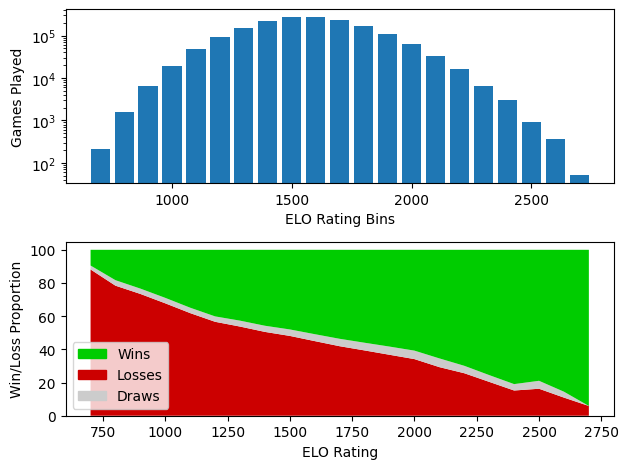
\includegraphics[scale=0.5]{Distribution and Win-Loss Proportion by ELO.png}}
\caption{Games Played vs. ELO Rating Bins (top): A bar chart showing the number of games played in each ELO rating range.
Win/Loss/Draw Proportions vs. ELO Rating (bottom): A stacked area chart visualizing the proportions of wins (green), losses (red), and draws (gray) for each ELO rating range.}
\label{fig}
\end{figure}

\subsection{Clustering Implementation}
 The cleaned dataset is used to group games based on player performance. The program applies the k-means clustering algorithm, leveraging Elo ratings as the primary axis for separation. Key steps include:
\begin{itemize}
    \item Determining the number of clusters(k): Using silhouette scores, the optimal value for k is selected, ensuring well-defined groupings.
    \item Running k-means: the algorithm partitions the data into clusters, where each cluster represents a subset of games with similar Elo ranges and gameplay characteristics.
\end{itemize}

\subsection{Statistical Analysis and Visualization}
After clustering the dataset, statistical analyses and visualization are performed to interpret the relationship between Elo ratings, game results, and gameplay patterns. these analyses highlight trends across different skill levels and provide actionable insight into the dataset.


\section{Experimental Setup}
\subsection{Dataset}
Original data can be accessed under the open database at Lichess.org. This is a very good source of raw record data for chess games, such as several billion games within the Lichess platform. It maintains metadata about the players' ratings, time controls, and outcomes, along with full move sequences in PGN format. The database is a treasure for research due to its size, diversity, and good accessibility; material on most types of games and all skill levels from beginners through grandmasters is covered.

In this project, only a subset of the data will be selected to demonstrate how some standard features like Rating, Total Move Count, and Outcome enable some effective clustering analysis. The data is already in structured PGN format; therefore, parsing and feature extraction will be easier. It will be ideal for exploring patterns and trends occurring in the play of chess.

This is documented in greater detail below, especially in Table 1, which outlines the structure and content of the files that make up the dataset.

\begin{table}[htbp]
\vspace{.01cm}
\caption{}
\begin{center}
\begin{tabular}{|lllll|}
\hline
\multicolumn{5}{|c|}{lichess.org dataset}                                                                                                      \\ \hline
\multicolumn{1}{|l|}{White name}  & \multicolumn{1}{l|}{Black name} & \multicolumn{1}{l|}{Result} & \multicolumn{1}{l|}{White Elo} & Black Elo \\ \hline
\multicolumn{1}{|l|}{paul2chess3} & \multicolumn{1}{l|}{Andique}    & \multicolumn{1}{l|}{1-0}    & \multicolumn{1}{l|}{1509}      & 1623      \\ \hline
\multicolumn{1}{|l|}{Shenhewho}   & \multicolumn{1}{l|}{Gentux}     & \multicolumn{1}{l|}{1-0}    & \multicolumn{1}{l|}{1857}      & 1963      \\ \hline
\end{tabular}
\begin{minipage}{8cm}
    \vspace{0.1cm}
    \small The table above shows 2 games from the dataset showing the payer names, the result of the game, and each player elo. there is other data included within the file but most of it is nonsense.
\end{minipage}
\end{center}
\end{table}

\subsection{Evaluation Metrics}
Quality clustering for the PGN project was made using some different metrics; among them, the most important was the silhouette score since this score gives a measure of how well the clusters are kept apart, and how well the game fits within its assigned cluster. In that way, clusters reflect real differences in either the level of players or their style of play. Additionally, inertia (within-cluster sum of squares) was used to evaluate the compactness of data points within clusters. Cluster size distribution was analyzed to identify any imbalances or outliers affecting the clustering process. To ensure the clusters' interpretability, we compared results against logical groupings, such as player rating ranges or typical game lengths, confirming that the clusters provided insight into game dynamics. These also allow us to assess the performance of our approach against overall simpler baselines such as rating-only clustering.

\subsection{Baseline}
The baselines were necessary for giving a comparison to the effectiveness of the clustering methodology on PGN data. A simple baseline entails the grouping of chess games regarding players' ratings into pre-defined ranges of cut-off, for instance, beginning, intermediate, and advanced players. This was a simplified comparison that didn't give a deep scope on how other features such as game length and its outcome interact. Other baselines were k-means clustering on fewer features for further benchmark performance checks. Comparing those with our multi-feature clustering methodology, we could then illustrate the advantages of integrating diverse features for nuanced gameplay. Since we were on the free version of Google Colab, runtime and memory needed to be optimized for baseline testing to do efficient experiments within resource bounds.

\subsection{Implementation Details}
The PGN clustering project has been developed in Python using the libraries: numpy for numerical operations, matplotlib for visualization, and sklearn to apply k-means clustering. For PGN elaboration, a personal parser has been used to extract relevant features from each match: players' ratings, total moves, and game outcomes. Then, data normalization was performed for correct clustering, while missing values were treated by deleting incomplete games. Therefore, k-means implementation was employed for the structured dataset, while the number of clusters was determined by the elbow method and silhouette score for the best performance. All the computations have been done on the free version of Google Colab, where computational resources were good enough to run this clustering analysis, though sometimes very limiting regarding duration and hardware.

\subsection{Hyper parameters}

\subsection{Figures and Tables}\label{}
\paragraph{Positioning Figures and Tables} Place figures and tables at the top and 
bottom of columns. Avoid placing them in the middle of columns. Large 
figures and tables may span across both columns. Figure captions should be 
below the figures; table heads should appear above the tables. Insert 
figures and tables after they are cited in the text. Use the abbreviation 
``Fig.~\ref{fig}'', even at the beginning of a sentence.

\section{results and discussion}

\section{Conclusion}

Figure Labels: Use 8 point Times New Roman for Figure labels. Use words 
rather than symbols or abbreviations when writing Figure axis labels to 
avoid confusing the reader. As an example, write the quantity 
``Magnetization'', or ``Magnetization, M'', not just ``M''. If including 
units in the label, present them within parentheses. Do not label axes only 
with units. In the example, write ``Magnetization (A/m)'' or ``Magnetization 
\{A[m(1)]\}'', not just ``A/m''. Do not label axes with a ratio of 
quantities and units. For example, write ``Temperature (K)'', not 
``Temperature/K''.

\begin{thebibliography}{00}
\bibitem{b1} F. Wijayanto, "Clustering Analysis of Chess Portable Game Notation Text," Jurnal Sians, Nalar, Dan Aplikasi Teknologi Informasi, 3(3), pp. 137--142, 2024.
\bibitem{b2} K. Raghav and L. Ahuja, "Chess Opening Analysis Using DBSCAN Clustering and Predictive Modeling," 2024 11th International Conference on Reliability, Infocom Technologies and Optimization (Trends and Future Directions) (ICRITO), Noida, India, 2024, pp. 1-5.
\bibitem{b3} C. Bauckhage, A. Drachen, and R. Sifa, "Clustering Game Behavior Data." IEEE Transactions on Computational Intelligence and AI in Games 7 (3).
\bibitem{b4} *Change* S. Shukla and N. S., "A Review ON K-means DATA Clustering APPROACH," .
\bibitem{b5} *Change* R. Nicole, ``Title of paper with only first word capitalized,'' J. Name Stand. Abbrev., in press.
\bibitem{b6} *Change* Y. Yorozu, M. Hirano, K. Oka, and Y. Tagawa, ``Electron spectroscopy studies on magneto-optical media and plastic substrate interface,'' IEEE Transl. J. Magn. Japan, vol. 2, pp. 740--741, August 1987 [Digests 9th Annual Conf. Magnetics Japan, p. 301, 1982].
\bibitem{b7} *Change* M. Young, The Technical Writer's Handbook. Mill Valley, CA: University Science, 1989.
\bibitem{b8} *Change* D. P. Kingma and M. Welling, ``Auto-encoding variational Bayes,'' 2013, arXiv:1312.6114. [Online]. Available: https://arxiv.org/abs/1312.6114
\bibitem{b9} *Change* S. Liu, ``Wi-Fi Energy Detection Testbed (12MTC),'' 2023, gitHub repository. [Online]. Available: https://github.com/liustone99/Wi-Fi-Energy-Detection-Testbed-12MTC
\bibitem{b10} *Change* ``Treatment episode data set: discharges (TEDS-D): concatenated, 2006 to 2009.'' U.S. Department of Health and Human Services, Substance Abuse and Mental Health Services Administration, Office of Applied Studies, August, 2013, DOI:10.3886/ICPSR30122.v2
\end{thebibliography}

\end{document}
